%!TEX root = main.tex
Assume a set of real numbers $\Omega = \{x_1, \ldots, x_N\}$ 
with cardinality $N$, where $x_1 \leq x_2 \leq \ldots, x_N$.
Without loss of generality, assume 
that all real numbers in $\Omega$ are 
in $[0, 1]$. 

The goal is to find an partition $\setI = \{I_j\}_{j = 1}^s$ of $[0, 1]$ into $s$ disjoint intervals, so that if we quantize every $x \in I_j$ to an endpoint of $I_j$, the variance is minimal over all possible partitions of $[0, 1]$ into $s$ intervals.
Formally:

\begin{align}
\nonumber \min_{\setI: |\setI| = s} \quad & \mathcal{MV}(\setI) := {1\over N}\sum_{j = 1}^s \sum_{x_i \in I_j} \err(x_i, I_j)\\
\text{s.t.}\quad & \bigcup_{j = 1}^s I_j = [0, 1].
\label{eq:opt_Q}
\end{align}

where $\err (x, I) = (b - x) (x - a)$ is the variance for point $x \in I$ if we quantize $x$ to an endpoint of $I = [a, b]$.
That is, $\err (x, I)$ is the variance of the (unique) distribution $D$ supported on ${a, b}$  so that $\E_{X \sim D} [X] = x$.


%\begin{align}
%\nonumber \min_{l_1, \cdots, l_{s-1}} \quad & \mathcal{MV}(l_1,\cdots, l_{s-1}) := {1\over N}\sum_{x\in \Omega} \sum_{k=1}^s {\bf 1}_k(x)V_k(x)\\
%\text{s.t.}\quad & 0 = l_0 \leq l_1\leq l_2 \leq \cdots \leq l_{s-1} \leq l_s = 1.
%\label{eq:opt_Q}
%\end{align}

Given an interval $I \subseteq [0, 1]$, we let $\setX_I$ be the set of $x_j \in \setX$ contained in $I$.
We also define $\err (\setX, I) = \sum_{x_j \in I} \err (x_j, I)$.
Given a partition $\setI$ of $[0, 1]$, we let $\err (\setX, \setI) = \sum_{I \in \setI} \err (\setX, I)$.
We also let $\setI^* = \argmin_{|\setI| = k} \err (\setX, \setI)$ (if there are multiple, then choose one arbitrarily), and we let $\OPT_s = \err(\setX, \setI^*)$.

The following lemma allows us to discretize the problem:
\begin{lemma}
There is a $\setI^*$ so that all endpoints of any $I \in \setI^*$ are in $\Omega \cup \{0, 1\}$.
\end{lemma}

\iffalse
\begin{proof}
Fix any endpoint $b$ of intervals in $\setI^*$.
WLOG assume that $b \neq 0, 1$.
Then we must have $I = [a, b]$ and $I' = [b, c]$ for some $I, I' \in \setI^*$.
Observe that the choice of $b$ only affects the error for points in $I \cup I'$.
We have that $\err (\Omega, I) + \err (\Omega, I') $ is given by
\begin{align*}
& \sum_{x \in I} (b - x) (x - a) + \sum_{x \in I'} (c -x)(x - b) \\
&= A b + C \; ,
\end{align*}
where $A, C$ are constants which do not depend on $b$.
Hence, this is a linear objective in $b$.
Since $b$ can freely range between the rightmost point in $I$ and the leftmost point in $I'$, there is an optimizer for this solution at one of those two points.
Hence we may choose $b \in \Omega$.
\end{proof}
\fi

Thus, it suffices to look for partitions who have endpoints at the points in our set.
This allows us to bring to bear combinatorial optimization techniques to this problem.

%The goal is to find  
%the optimal set of $s$ quantization 
%levels $\{l_1, l_2, \cdots, l_{s-1}\}$ 
%which minimize the mean quantization variance. Formally:
%\begin{align}
%\nonumber \min_{l_1, \cdots, l_{s-1}} \quad & \mathcal{MV}(l_1,\cdots, l_{s-1}) := {1\over N}\sum_{x\in \Omega} \sum_{k=1}^s {\bf 1}_k(x)V_k(x)\\
%\text{s.t.}\quad & 0 = l_0 \leq l_1\leq l_2 \leq \cdots \leq l_{s-1} \leq l_s = 1.
%\label{eq:opt_Q}
%\end{align}
%where ${\bf 1}_k(x)$ is the indicator function
%\[
%{\bf 1}_k(x) = 
%\begin{cases}
%1 & \text{if}~x\in (l_{k-1}, l_k] \\
%0 & \text{o.w.}
%\end{cases}
%\]
%and $V_k(x)$ is the variance function 
%\begin{align}
%V_k(x) = (x-p_{k-1})(p_k - x), \label{eq:var}
%\end{align}
%which is the variance of Bernoulli distribution with probability $l_k-x$ taking value $l_{k-1}$ and probability $x-l_{k-1}$ taking value $l_k$. ${\bf 1}_k(x)V_k(x)$ is the variance if $x$ falls into the interval $(l_{k-1}, l_k]$. 

%This problem is hard to solve directly, due to non-convexity and non-smoothness. We discretize the range $[0,1]$ into $M$ intervals, i.e., $[0,d_1), [d_1, d_2), \cdots, [d_{M-1}, 1]$ with $0< d_1<d_2<\cdots < d_{M-1}<1$. All $l_k$'s are restricted to values in $\{d_1, d_2, \cdots, d_{M-1}\}$ while satisfying  monotonicity. 
%
%\begin{theorem} \label{thm:optQ}
%Let the maximal number of data points in each ``small interval'' (defined by $\{d_m\}_{m=1}^{M-1}$) and the maximal length of small intervals be bounded by $bN/M$ and $a/M$, respectively. Let $\{l^*_k\}_{k=1}^{s-1}$ and $\{\hat{l}^*_k\}_{k=1}^{s-1}$ be the optimal quantization to \eqref{eq:opt_Q} and the solution with discretization. Let $cM/s$ be the upper bound of the number of small intervals crossed by any ``large interval'' (defined by $\{l^*_k\}_{k=1}^{s-1}$). Then we have the discretization error bounded by
%\[
% \mathcal{MV}(\hat{l}^*_1,\cdots, \hat{l}^*_{s-1}) -  \mathcal{MV}(l^*_1,\cdots, l^*_{s-1}) \leq {a^2b s \over 4 M^3} + {a^2bc^2 \over Ms}.
%\]
%\end{theorem}
%
%Note that if the numbers of data points falling into all small intervals are equal, then
%the constant $b$ is $1$. So $b$ roughly measures the uniformness of the data distribution w.r.t. small intervals. If all small intervals have equal length, then $a$ is equal to $1$. So $a$ roughly measures the distortion from equal-length small intervals. 
%Similarly, $c$ roughly measures the distortion from equal-length large intervals since $c=1$ means that all large intervals defined by $\{l^*_k\}_{k=1}^{s-1}$ roughly cross the same number of small intervals defined by $\{d_m\}_{m=1}^{M-1}$. Theorem~\ref{thm:optQ} suggests that the mean variance using the discrete variance-optimal quantization will converge to the optimal with the rate $O(1/Ms)$.

\begin{figure}[t]
\centering    
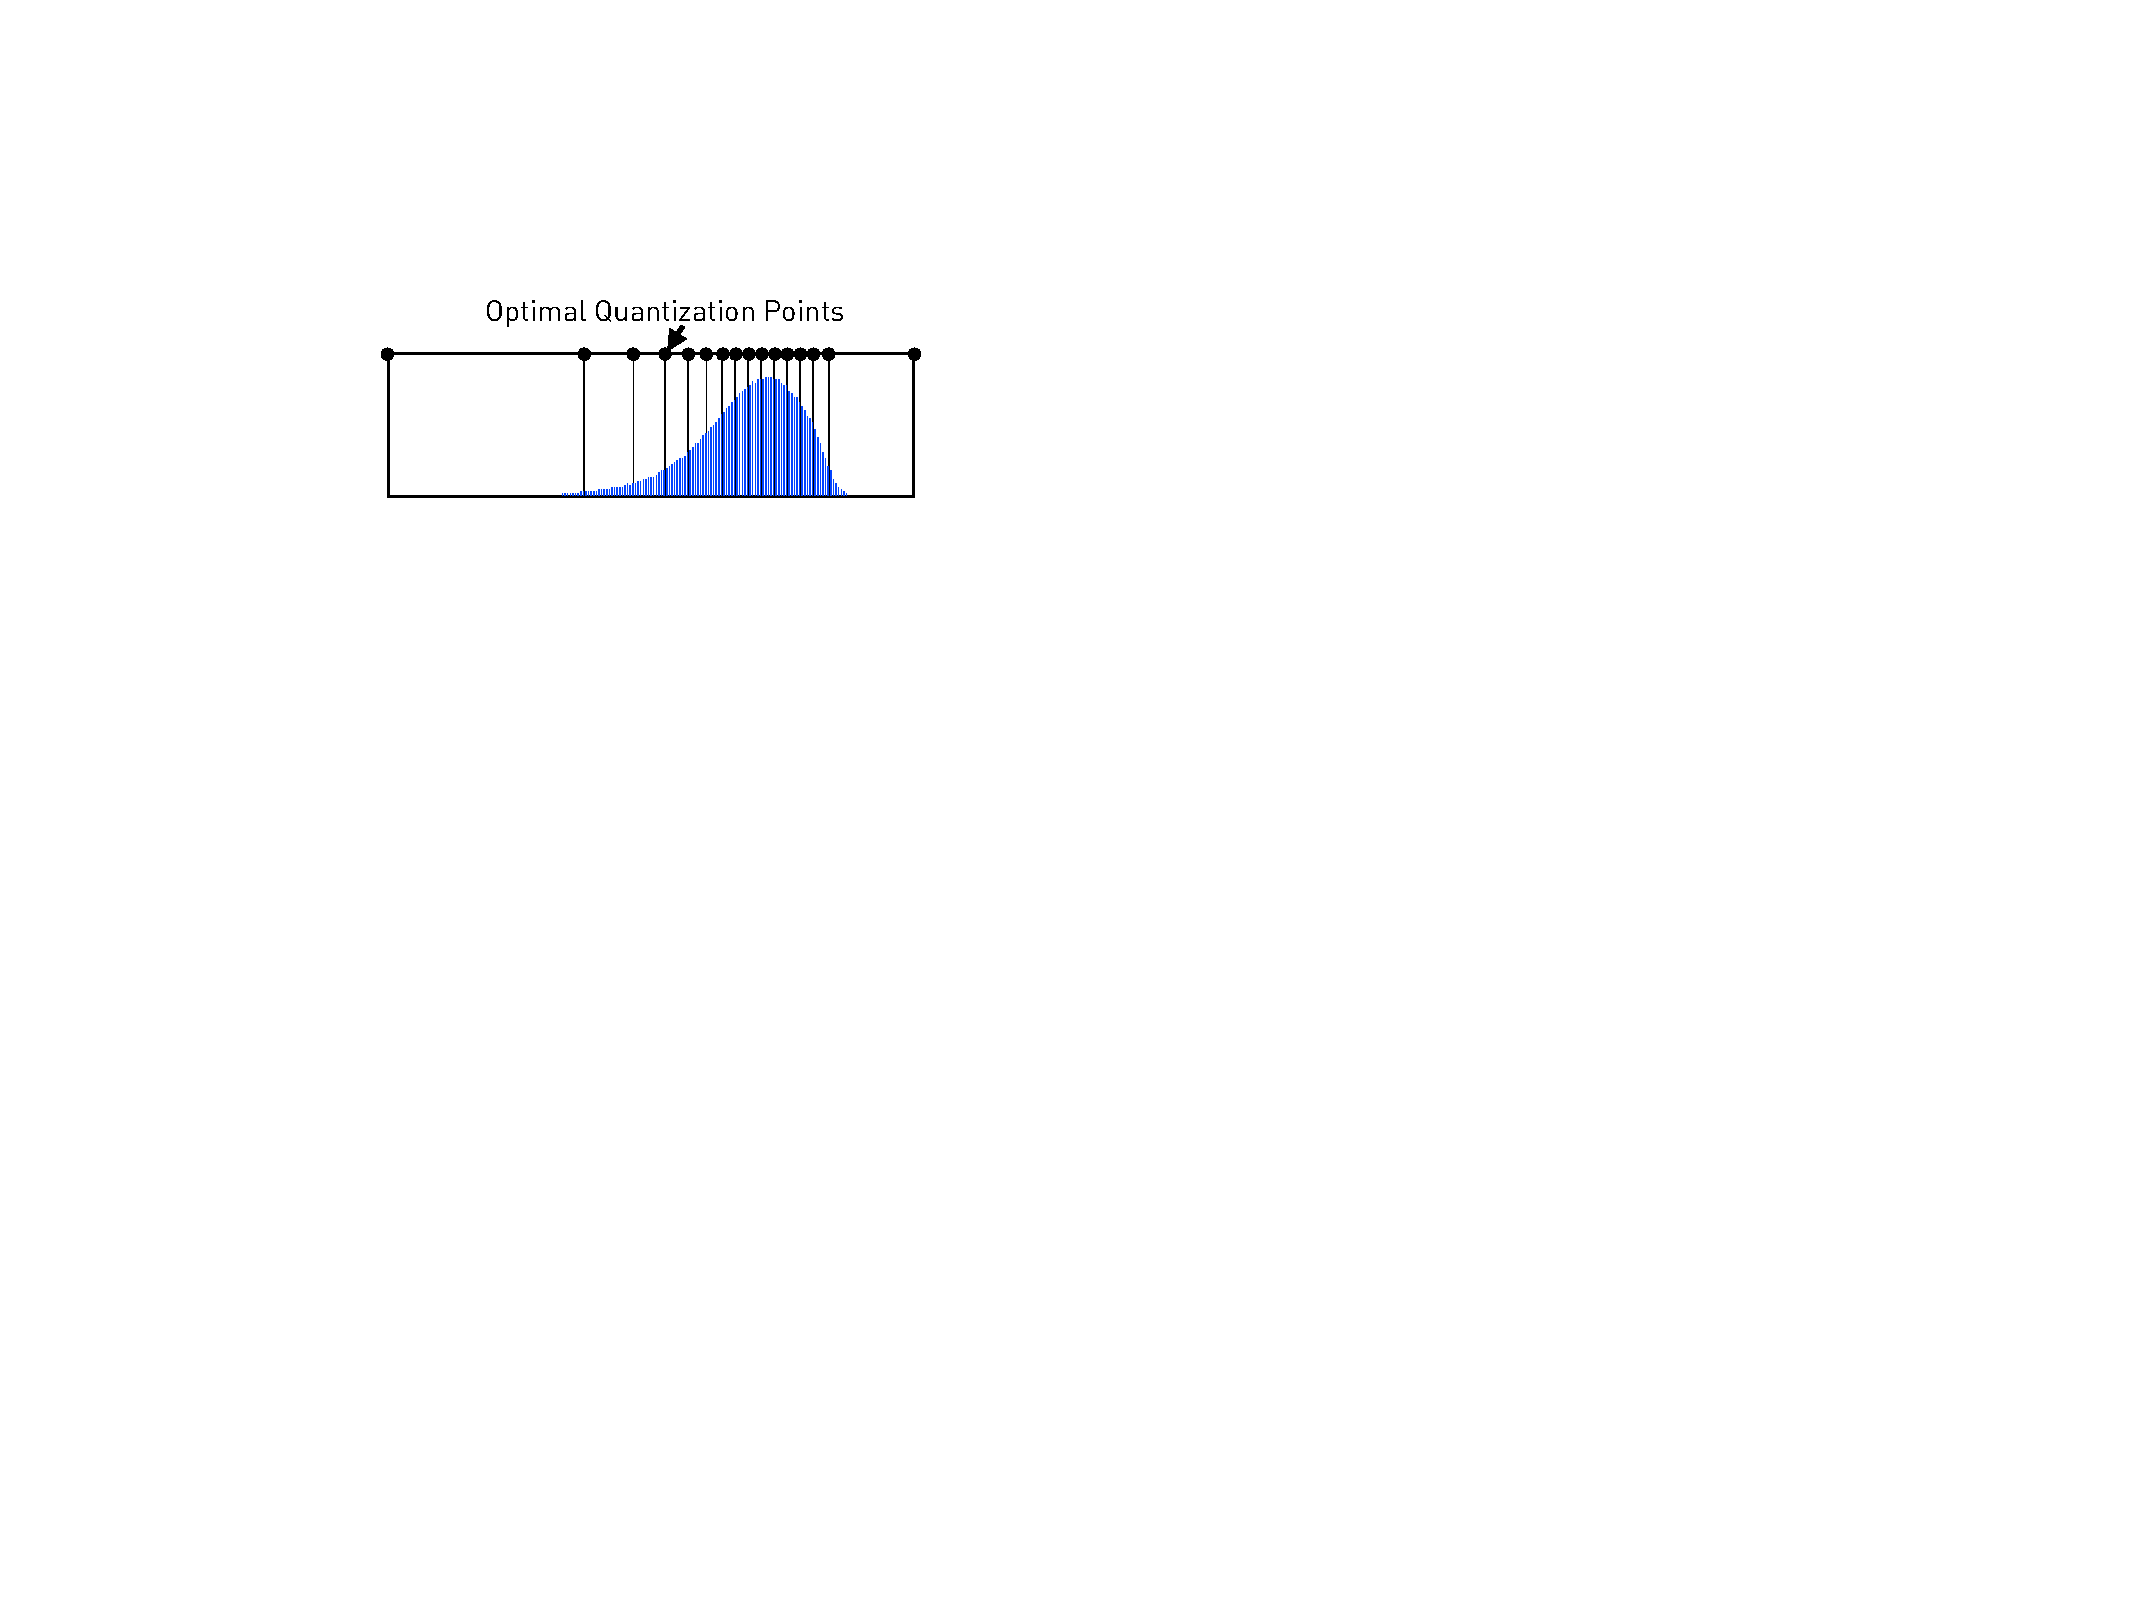
\includegraphics[width=0.7\columnwidth]{micro-experiments/dp-level.pdf} 
\caption{Optimal quantization points calculated with
dynamic programming given a data distribution. }
\label{fig:optimalquantization}
\end{figure} 

\paragraph*{Dynamic Programming}

We describe
a dynamic programming algorithm to 
find the optimal solution.

Define $T(k, m)$ be the optimal total variance for points in $[x_1, x_m]$ with $k$ quantization levels. Our goal is to calculate $T(s, N)$. This problem can be solved by dynamic programing using the following recursion
\[
T(k, m) = \min_{j\in \{k-1, k, \cdots, m-1\}} T(k-1,j) + \err (\Omega, [x_j, x_m]).
\]
The term $\err (\Omega, [x_j, x_m])$ can obviously be computed in linear time, and so the time complexity of this program is dominated by the complexity of filling in $T(\cdot, \cdot)$, which is $O(s N^2)$.
After filling in this matrix, we can find the optimal partition by classical backtracking techniques.

Figure~\ref{fig:optimalquantization} illlustrates
an example output for our algorithm.

%\paragraph*{Approximate dynamic programming}
%This program requires quadratic time in $N$ to run, which is often infeasible in practice.
% We discretize the range $[0,1]$ into $M$ intervals, i.e., $[0,d_1), [d_1, d_2), \cdots, [d_{M-1}, 1]$ with $0< d_1<d_2<\cdots < d_{M-1}<1$. All $l_k$'s are restricted to values in $\{d_1, d_2, \cdots, d_{M-1}\}$ while satisfying  monotonicity. 
%
%\begin{theorem} \label{thm:optQ}
%Let the maximal number of data points in each ``small interval'' (defined by $\{d_m\}_{m=1}^{M-1}$) and the maximal length of small intervals be bounded by $bN/M$ and $a/M$, respectively. Let $\{l^*_k\}_{k=1}^{s-1}$ and $\{\hat{l}^*_k\}_{k=1}^{s-1}$ be the optimal quantization to \eqref{eq:opt_Q} and the solution with discretization. Let $cM/s$ be the upper bound of the number of small intervals crossed by any ``large interval'' (defined by $\{l^*_k\}_{k=1}^{s-1}$). Then we have the discretization error bounded by
%\[
% \mathcal{MV}(\hat{l}^*_1,\cdots, \hat{l}^*_{s-1}) -  \mathcal{MV}(l^*_1,\cdots, l^*_{s-1}) \leq {a^2b s \over 4 M^3} + {a^2bc^2 \over Ms}.
%\]
%\end{theorem}
%

%where $V(j,m)$ denotes the total variance of points falling into the interval $[d_j, d_m]$. 
%The optimal value for $l_{s-1}^*$ is $ d_{j^*_{s-1}}$ with $j^*_{s-1}$ equal to
%\[
%j^*_{s-1} = \argmin_{j\in \{s-1, k, \cdots, M-1\}} T(s-1,j) + V(j,M),
%\]
%and the rest can be retrieved by 
%\begin{align*}
%j^*_{k-1} = \argmin_{j\in \{k-1, k, \cdots, j^*_k-1\}} T(k-1, j) + V(j, j^*_k) \\
%\text{for all}~k=2, \cdots, K-2
%\end{align*}

%The complexity of calculating the matrix $V(\cdot, \cdot)$ is $O(M^2 + N)$ and the complexity of calculating matrix $T(\cdot, \cdot)$ is $O(sM^2)$. The total memory cost is $O(sM + M^2)$. Note that to find the optimal quantization, we only need to scan all $N$ numbers once.
%The calculation of $V$ is not trivial (it needs
%another dynamic programming algorithm) and we
%describe the details in the full version.

%Define $T(k, m)$ be the optimal total variance for points in $[0, d_m]$ with $k$ quantization levels. Our goal is to calculate $T(s, M)$. This problem can be solved by dynamic programing using the following recursion
%\[
%T(k, m) = \min_{j\in \{k-1, k, \cdots, m-1\}} T(k-1,j) + V(j,m),
%\]
%where $V(j,m)$ denotes the total variance of points falling into the interval $[d_j, d_m]$. The optimal value for $l_{s-1}^*$ is $ d_{j^*_{s-1}}$ with $j^*_{s-1}$ equal to
%\[
%j^*_{s-1} = \argmin_{j\in \{s-1, k, \cdots, M-1\}} T(s-1,j) + V(j,M),
%\]
%and the rest can be retrieved by 
%\begin{align*}
%j^*_{k-1} = \argmin_{j\in \{k-1, k, \cdots, j^*_k-1\}} T(k-1, j) + V(j, j^*_k) \\
%\text{for all}~k=2, \cdots, K-2
%\end{align*}
%
%The complexity of calculating the matrix $V(\cdot, \cdot)$ is $O(M^2 + N)$ and the complexity of calculating matrix $T(\cdot, \cdot)$ is $O(sM^2)$. The total memory cost is $O(sM + M^2)$. Note that to find the optimal quantization, we only need to scan all $N$ numbers once.
%The calculation of $V$ is not trivial (it needs
%another dynamic programming algorithm) and we
%describe the details in the full version.
%Figure~\ref{fig:optimalquantization} illlustrates
%an example output for our algorithm.


\iffalse
\begin{proof}
Let $p^*_0$ be $0$ and $p^*_K=1$.We quantitize $\{p^*_k\}_{k=1}^{K-1}$ one element by one element, while monitor the changing of the total variance $N \times \mathcal{MV(\cdot)}$. We first quantize $p^*_1$ to the closest value (denoted it by $Q(p^*_1)$) in $\{d_m\}_{m=1}^{M-1} \cup \{p^*_0,p^*_K\}$ under the monotonicity constraint, that is, $p^*_0\leq Q(p^*_1) \leq p^*_2$. Here, one important observation is $|p^*_{1} - Q(p^*_1)|\leq a/M$. Consider the total variance of this new solution $Q(p^*_1), p^*_2, \cdots, p^*_{K-1}$. The variance of points falling into the range $[p^*_2, 1]$ does not change at all. Without the loss of generality, assume $p^*_{1} \geq Q(p^*_1)$.

Next we consider points falling into the following three sets $C_1 = [p^*_0, Q(p^*_1)]$, $C_2 = [Q(p^*_1), p^*_1]$, and $C_3 = [p^*_1, p^*_2]$. The variance of points of falling into $C_1$ gets reduced from the form of variance in \eqref{eq:var}. Next we only need to check the variance change for points in $C_2$ and $C_3$. Consider $C_2$ first. The variance for point $x$ in $C_2$ is
\[
(x-Q(p^*_1))(p^*_1 - x) \leq {a^2 \over 4 M^2}. 
\]  
Thus, the change of variance for points in $C_2$ would be bounded by ${a^2 \over 4 M^2}$. Then consider $C_3$. The change of variance for point $x$ in $C_3$ is
\begin{align*}
& (x-Q(p^*_1))(p^*_2 - x) - (x-p^*_1) (p^*_2 - x) 
\\
= & (p^*_1 - Q(p^*_1)) (p^*_2 - x)
\\
\leq & {a\over M}(p^*_2 - x)
\end{align*}
Therefore, the change of total variance from $\{p^*_1, p^*_2, \cdots, p^*_{K-1}\}$ to $\{Q(p^*_1), p^*_2, \cdots, p^*_{K-1}\}$ is bounded by 
\begin{align}
\nonumber
& \sum_{x\in C_2} {a^2 \over 4M^2} + \sum_{x \in C_3} {a\over M}(p^*_2 - x)
\\
\nonumber
\leq & {Nb \over M} {a^2 \over 4M^2} + {a\over M}{Nb \over M} \sum_{t=1}^{cM/K}t{a\over M}
\\
\leq &
{a^2b N \over 4 M^3} + {a^2bc^2 N \over MK^2}
\label{eq:bound_1step}
\end{align}
Similarly, we quantitize $p^2_2$ in $\{Q(p^*_1), p^*_2, \cdots, p^*_{K-1}\}$ to get a new solution $\{Q(p^*_1), Q(p^*_2), \cdots, p^*_{K-1}\}$ while maintain the monotonicity. We can establish the same upper bound to \eqref{eq:bound_1step}. Following this idea, we can obtain a quantization solution $\{Q(p^*_1), Q(p^*_2), \cdots, Q(p^*_{K-1})\}$. Therefore, we obtain that 
\begin{align*}
&  \mathcal{MV}(Q(p^*_1), Q(p^*_2), \cdots, Q(p^*_{K-1})) -  \mathcal{MV}({p}^*_1,\cdots, {p}^*_{K-1}) 
 \\
 & \quad \leq {a^2b K \over 4 M^3} + {a^2bc^2 \over MK}.
\end{align*}
Using the fact that $ \mathcal{MV}(p^*_1,\cdots, p^*_{K-1})$ is smaller than $\mathcal{MV}(Q(p^*_1), Q(p^*_2), \cdots, Q(p^*_{K-1}))$ proves the claim.
\end{proof}
\fi

\paragraph*{A Greedy Approximation Algorithm}
We now describe a nearly linear time algorithm for this problem, which we can show is provably competitive with the optimal solution.
This algorithm is very similar to one by \cite{ADHLS15} for the histogram recovery problem.

Our algorithm, at a high level, proceeds as follows.
Suppose we wish to compete with the best quantization that uses $k$ points.
Initially, we form the partition $\setI$ so that each point in $\setX$ is in its own interval.
Then, we repeatedly do the following procedure:
\begin{enumerate}
\item
Pair up consecutive intervals in the partition, so that we form $|\setI| / 2$ ``candidate'' intervals, which we propose to merge.
For each such candidate interval $J$, compute $\err(\setX, J)$.
\item
Find the $2 s$ candidate intervals with largest $\err (\setX, J)$.
Do not merge these intervals, and merge the remaining.
\end{enumerate}

We defer the formal pseudocode of this to the full version.
Each step requires only a single pass through the data.
Moreover, we show in the full version that we can do at most logarithmically many iterations.
Thus, the algorithm runs in nearly linear time.
In the full version of the paper, we show:
\begin{theorem}
Given any $\setX, k$, let $\setI$ be the output of the above algorithm.
Then $\setI$ has at most $4s + 1$ intervals, and we have that $\err (\setX, \setI) \leq 2 \OPT_s$.
\end{theorem}
We can tune these parameters, to get a tradeoff between how many intervals remain, and how much error we tolerate.
Moreover, to get the output of the algorithm down to size exactly $s$, we may also do an additional dynamic programming postprocessing routine on the output of this algorithm.
This postprocessing now looks for the best partition with $s$ pieces at endpoints given by endpoints of $\setI$, and so runs in time $O(s^2 N)$, i.e., nearly-linear in the number of samples.

%We require the following lemma, whose proof is trivial and omitted.
%\begin{lemma}
%If $I \subseteq I'$, then $\err(\setX, I) = \err (\setX_I, I) \leq \err (\setX_I, I')$.
%\end{lemma}









